\documentclass[12pt,a4paper,twoside,openright,fleqn]{mwrep}
\usepackage[utf8]{inputenc}
\usepackage[OT4,plmath]{polski}
\usepackage{amsmath}
\usepackage{amssymb}
\usepackage{graphicx}
%\usepackage[a4paper,left=3.5cm,right=2.5cm,top=2.5cm,bottom=2.5cm]{geometry}
\usepackage[width=16cm,height=25cm]{geometry}
\usepackage{fancyvrb}
\usepackage{listings}
%\usepackage{bold-extra}
\usepackage[unicode=true]{hyperref}
\usepackage{color}
\usepackage{cite}

\pagestyle{uheadings}

% Definicje ustalaj±ce wygl±d wydruków programów
\definecolor{darkgray}{rgb}{0.95,0.95,0.95}
\lstset{frame=tb, backgroundcolor=\color{darkgray}}
\lstset{numbers=left, numberstyle=\tiny, stepnumber=2, numbersep=5pt}
\lstset{basicstyle=\ttfamily, keywordstyle=\color{blue}\bfseries}


%\hypersetup{
%    pdfpagemode=UseOutlines,   % otwiera dokument w trybie jednej strony
%    pdfpagelayout=SinglePage,  %
%    pdfstartpage=1,            % na podanej stronie
%    bookmarksopen=true,        % rozwiniêcie zak³adek
%    bookmarksopenlevel=1,   % do jakiego poziomu
%    colorlinks=true,   % kolorowanie odno¶ników zamiast ramki wokó³ nich
%    citecolor=cyan,   % kolor odno¶ników do bibliografii, domy¶lnie zielony
%    filecolor=red,   % kolor odno¶ników do lokalnych plików, domy¶nie magenta
%    linkcolor=blue,   % kolor odno¶ników wewnêtrznych, domy¶lnie czerwony
%    menucolor=green,   % kolor pozycji menu Acrobata, domy¶lnie czerwony
%    urlcolor=blue,   % kolor odno¶ników do adresów internetowych, domy¶lnie cyan
%                               % DANE DOKUMENTACJI
%    pdfauthor={Mateusz Nowakowski},
%    pdftitle={Praca inżynierska},
%    pdfsubject={Lokalizacja robota klasy Micromouse w labiryncie},
%    pdfkeywords={Micromouse, micromouse}
% }

                                   % DEFINICJE W£ASNE
\newcommand{\dd}{\text{d}}
\newtheorem{uwaga}{Uwaga}
\newtheorem{twr}{Twierdzenie}


\title{Lokalizacja robota klasy Micromouse w labiryncie}
\author{Mateusz Nowakowski}
\date{\today}


\def\labelitemi{$\bullet$} 

\begin{document}

\VerbatimFootnotes

\maketitle

\tableofcontents

 \chapter{Wstęp} 
 \section{Cel projektu i zadania robota} 
 Celem projektu jest zaprojektowanie i implementacja algorytmów pozwalających na określenie pozycji robota klasy Micromouse w labiryncie. Robot musi być w stanie umiejscowić się w labiryncie, planować drogę do jego środka oraz podążać po wyznaczonej ścieżce odpowiednio filtrując odczyty z sensorów. W ramach projektu wykonano:
 \begin{itemize}
     \item komputerowy model robota 3D,
     \item płytkę elektroniki,
     \item schemat ideowy,
     \item prototyp robota,
     \item biblioteki do obsługi niezbędnych peryferii wybranego mikrokontrolera,
     \item system wizyjny do testowania jakości wykorzystywanych algorytmów,
 \end{itemize}

 
 \section{Robot klasy Micromouse}
 Celem konkurencji Micromouse jest pokonanie w jak najkrótszym czasie drogi od początku do środka labiryntu. Poprzez środek labiryntu rozumiemy kwadrat utworzony z czterech pól z jednym dojazdem. Każde pole ma wymiary 18 x 18 cm. Rozmiar robota ograniczony jest przez rozmiar jednego pola, waga robota jest nie ograniczenia. Omawiana konstrukcja musi być w pełni autonomiczna i nie może kontaktować się z żadnymi zewnętrznymi urządzeniami. W konkurencji oceniane są 2 przejazdy. Pierwszy którym robot uczy się labiryntu i stara się dojechać do jego końca. W drugim przejeździe robot powinien w jak najkrótszym czasie dojechać do środka labiryntu-- do tego celu wykorzystywana jest wiedza o labiryncie zdobyta podczas pierwszego przejazdu.

\begin{figure}[h]
\centering
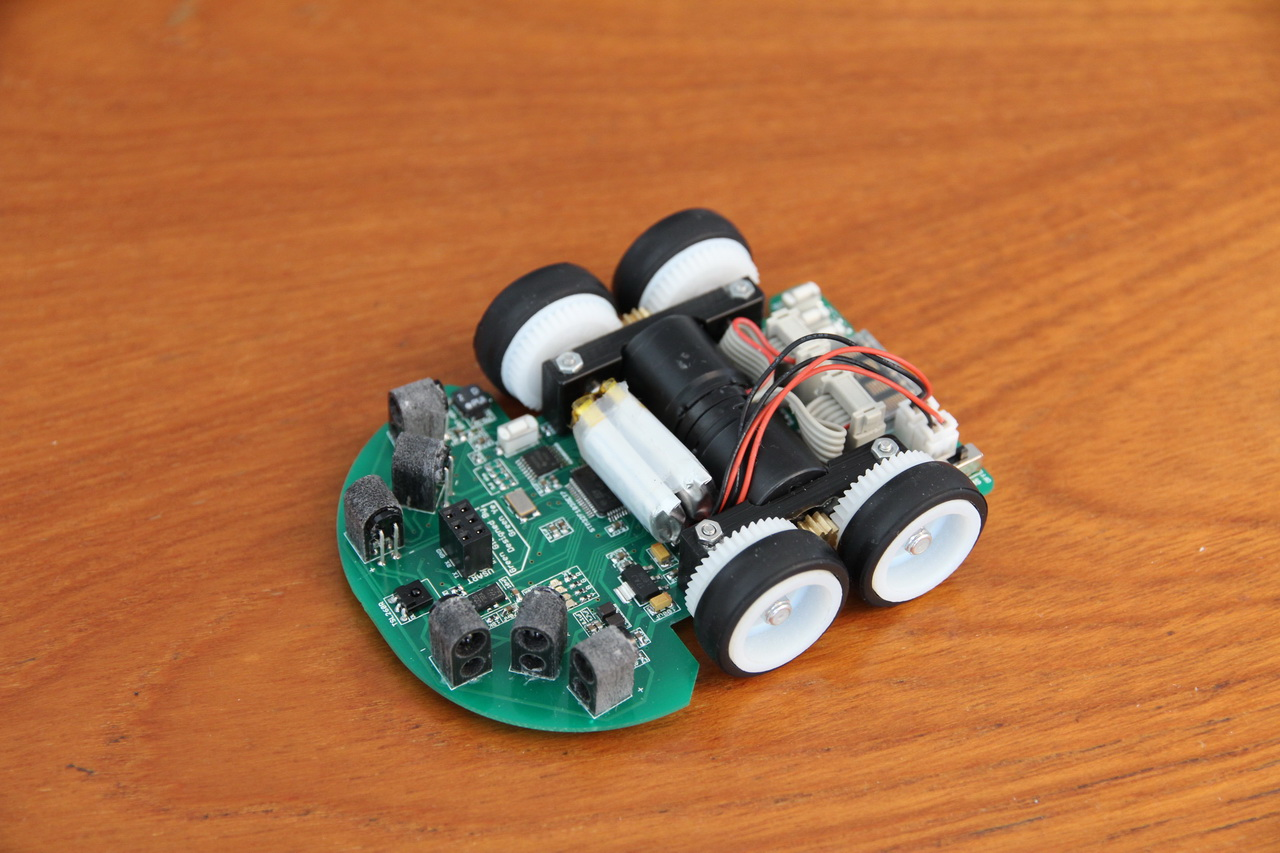
\includegraphics[width=0.5\textwidth]{./images/green_glant}
\caption{Robot Green-Glant}
\label{green_glant}
\end{figure}

\begin{figure}[h]
\centering
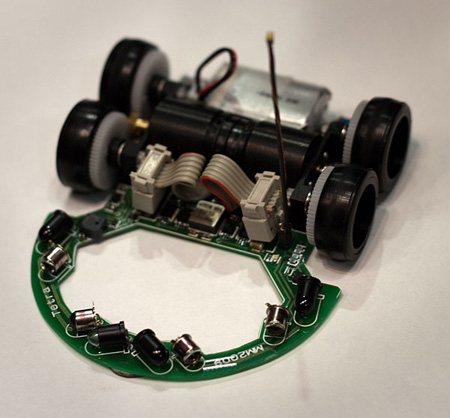
\includegraphics[width=0.5\textwidth]{./images/tetra}
\caption{Micromouse Tetra}
\label{tetra}
\end{figure}

\section{Przewidywane problemy} 

\subsection{Względność}
Dla robota klasy Micromouse występuje potrzeba monitorowanie takich parametrów jak orientacja i położenie. Ze względu na to, że robot nie posiada żadnych informacji z zewnątrz wszystkie informacje jakie gromadzi są informacjami względnymi -- w najlepszy przypadku posiada informacje o przesunięciu i obrocie względem pozycji początkowej. W przypadku zadania lokalizacji względem układu zewnętrznego jakim jest labirynt jest to zjawisko niepożądane ponieważ początkowe położenie robota może mieć znaczny wpływ na zachowanie robota. 

\subsection{Określanie orientacji robota} 
Określanie orientacji sprowadza się tak na prawdę do dwóch mniejszych problemów 

\begin{itemize}
    \item określania orientacji podczas obrotu 
    \item określania orientacji w celu utrzymania zadanej trajektorii ruchu
\end{itemize}

Dla robota klasy Micromouse wymagana jest kontrola i wiedza o aktualnym położeniu i orientacji robota. Wiedza ta jest niezbędna do nawigacji w labiryncie. Pozwala to na odpowiednie poruszanie się. Aby umożliwić kontrolę orientacji robota konieczne jest wyposażenie robota w odpowiednio szybkie, dokładne oraz odporne na zakłócenia czujniki. Przykładem  czujników umożliwiających ten parametr robota są enkodery lub żyroskop. 

Przy wykorzystywaniu żyroskopu należy zdawać sobie sprawę ze zjawiska jakim jest dryf żyroskopu. Zakłócenia generowane przez żyroskop w przypadku robota klasy Micromouse są ciężkie do wyeliminowania gdyż wartość dryf nie jest zakłóceniem losowym. 

Do pomiaru orientacji wykorzystano dwa rodzaje czujników: enkodery oraz żyroskop. Żaden z wykorzystanych czujników nie jest idealny. 

Alternatywą dla żyroskopu jest wykorzystanie enkoderów magnetycznych umieszczonych na kołach robota. Znając promień robota (wykorzystywania konstrukcja jest okrągłym robotem klasy 2.0 z symetrycznie umieszczonymi kołami jak na rysunku~\ref{robot_3d}) oraz promień koła robota można obliczyć drogę jaką muszą pokonać koła aby robot obrócił się o zadany kąt.

\begin{figure}[h]
\centering \includegraphics[width=0.7\textwidth]{./images/robot_3d}
\caption{model robota wykorzystywany w trakcie badań}
\end{figure}

\subsection{Określanie przejechanej drogi} % (fold)
Robot musi mieć możliwość pomiaru przejechanej drogi aby być w stanie określić swoją pozycje w labiryncie. Do realizacji tego typu pomiaru planuje się wewnątrz kół zamocować magnesy neodymowe,a do pomiaru przemieszczenia kół użyć enkoderów magnetycznych. W celu usprawnienia pomiarów pochodzących z enkoderów zdecydowano się na wykorzystanie mikrokontrolera ze sprzętową obsługą sygnału kwadraturowego. Metoda ta nie jest jednak idealna nie uwzględnia ona poślizgów kół robota oraz ugięcia się kół co może wprowadzać błędu przy określaniu pozycji robota. 


\subsection{Pomiar odległości oraz wykrywanie ścian labiryntu} % (fold)
W celu pomiaru odległości robota od ścian labiryntu jak i ich wykrywania należało wyposażyć robota w odpowiednie czujniki odległości. Umiejętność oceny przez robota jak daleko znajduje się od ściany labiryntu jest niezbędna do unikania kolizji ponadto czujniki te pozwalają na wykrywanie obecności ścian labiryntu. 

Ponadto czujniki te są jedynymi z czujników które wykorzystuje robot dającymi informacje o labiryncie i pomiary pochodzące z nich są najbardziej wiarygodne. Robot co prawda może posiadać informacje o budowie labiryntu oraz korzystając z wyżej wymienionych czujników aproksymować swoja pozycję jednakże to właśnie czujniki odległości pozwalają na weryfikację pomiarów. 

\subsection{Eliminacja poślizgów kół} % (fold)
Dużym problemem w robotach klasy Micromouse jest wykorzystywanie enkoderów. Wykorzystywany aparat matematyczny służący do wyznaczania drogi na podstawie odczytów z enkoderów nie uwzględnia w żaden sposób poślizgów kół robota. W celu ograniczenia wpływu tego czynnika na pomiary można zaimplementować trapezoidalny profil prędkości i dobrać takie kąty nachylenia profili prędkości narastania i hamowania aby zminimalizować możliwość występowania poślizgów. 

\section{Wpływ oświetlenia labiryntu na pomiary } % (fold)

Czujniki odległości zaprojektowano z wykorzystaniem fotodiody oraz fototranzystora. Pomimo, że wybrane podzespoły charakterystyką obejmuję jedynie bardzo mały obszar światła widzialnego okazało się iż zakłócenia generowane przez oświetlenie mają istotny wpływ na pomiary odległości i wykrywanie ścian labiryntu. 

% section Wpływ oświetlenia labiryntu na pomiary  (end)
\section{Sterowanie robotem klasy Micromouse} % (fold)

Celem robotów startujących w konkurencji Micromouse jest dojechanie do środka labiryntu. Aby robot był w stanie manewrować w labiryncie musi być w stanie wykonywać 2 podstawowe akcje:

\begin{itemize}
    \item obrót o zadany kąt 
    \item kontrola trajektorii podczas jazdy na wprost
    \item ruch w przód o zadaną odległość
\end{itemize}


Akcje te są wystarczające do tego aby nawigować w labiryncie, w celu optymalizacji czasu przejazdu labiryntu, możliwe jest wykorzystanie dodatkowych akcji takich jak jazda po łuku, która pozwala na płynniejsze pokonywanie zakrętów i nie wiąże się z koniecznością zatrzymywania robota podczas pokonywania zakrętów.

\subsection{Obrót o zadany kąt i kontrola trajektorii} % (fold)

Zadając obrót robota za pomocą enkoderów korzystamy z zależności, która pozwala nam wyliczyć drogę jaką muszą pokonać koła aby robot obrócił się o zadany kąt:

$$ f(x)=\frac{ k \cdot x \cdot  2\pi R}{360 \cdot 2 \pi r} $$


\begin{itemize}
    \item $f(x)$ -- ilość impulsów enkodera o jaką mają obrócić się koła 
    \item $x$ -- zadany kąt 
    \item $k$ -- ilość ticków enkodera na jeden obrót koła
    \item $R$ -- promień robota
        \begin{figure}[h]
        \centering
        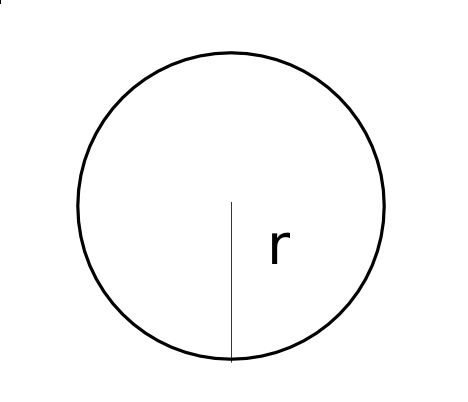
\includegraphics[width=0.4\textwidth]{./images/wheel_r}
        \caption{koło robota}
        \label{wheel_r}
        \end{figure}
    \item $r$ -- promień koła
        \begin{figure}[h]
        \centering
        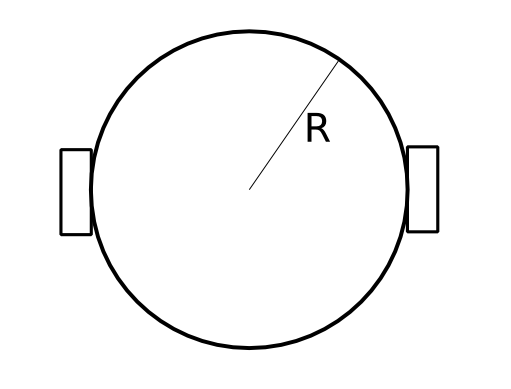
\includegraphics[width=0.4\textwidth]{./images/robot_r}
        \caption{robot}
        \label{robot_r}
        \end{figure}
\end{itemize}


Przy sterowaniu kątem obrotu z wykorzystaniem enkoderów, jako wymuszenie na regulator podawana jest droga kątowa jaką mają przebyć koła i droga ta porównywana jest z rzeczywistą odległością jaką przebyły. Informacja o aktualnej drodze uzyskiwana jest poprzez całkowanie impulsów pochodzących z enkoderów. 

\begin{figure}[h]
\centering
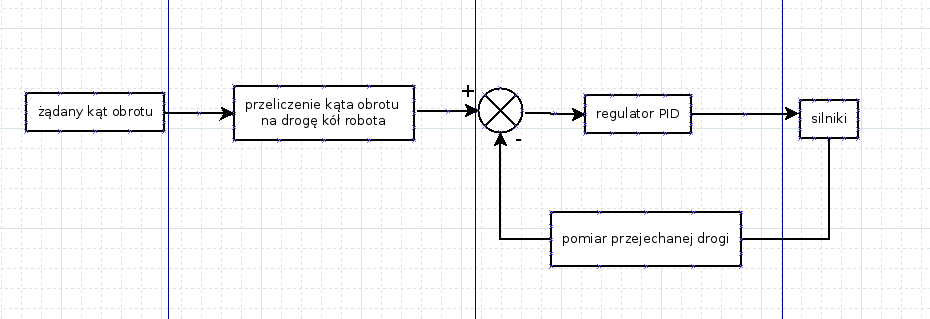
\includegraphics[width=1.0\textwidth]{./images/enkoder_uklad_sterowania}
\caption{schemat układu sterowania kąt obrotu z wykorzystaniem enkoderów}
\label{enkoder_uklad_sterowania}
\end{figure}


Sterowanie kątem obrotu za pomocą enkodera jest jednak niedokładne, wzór nie uwzględnia ugięcia się kół oraz możliwych poślizgów. O ile ugięcie kół możemy pominąć, to problem poślizgu może wprowadzać duże błędy w szacowaniu orientacji robota. 

Alternatywą do sterowania kątem obrotu za pomocą enkoderów może być sterowanie przy wykorzystaniu żyroskopu. W celu określania aktualnej pozycji korzystamy ze wzoru:

$$ x = \int_{t_0}^{t_1} \omega(t) dt $$

\begin{itemize}
   \item $x$ -- aktualne położenie kątowe
   \item $\omega(t)$ -- odczytana z żyroskopu prędkość kątowa
\end{itemize}

\begin{figure}[h]
\centering
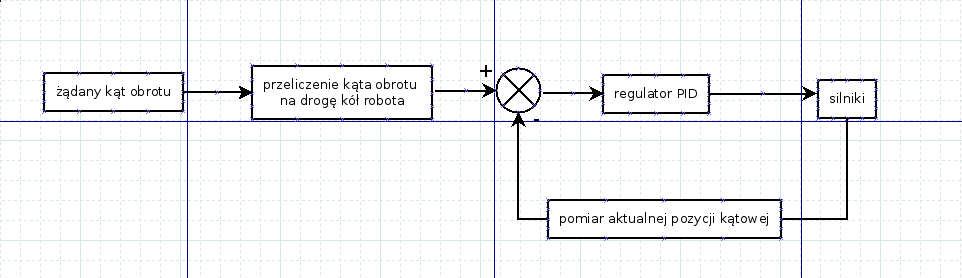
\includegraphics[width=1.0\textwidth]{./images/zyroskop_uklad_sterowania}
\caption{schemat układu sterowania kątem obrotu z wykorzystaniem żyroskopu}
\label{zyroskop_uklad_sterowania}
\end{figure}

Jednakże ze względu na naturę działania żyroskopu oraz fakt, że jest czujnikiem inercyjnym pojawia się tzw dryf żyroskopu, który wprowadza znaczne błędy. Ze względu na to żyroskop podczas pracy powinien być kalibrowany tak aby zminimalizować oddziaływanie dryfu na pomiary. Żyroskop również nie jest idealnym wyborem. 


\subsection{Ruch w przód o zadaną odległość} % (fold)

Jest to podstawowa akcja robota gdyż pozwala na przemieszczanie się robota pomiędzy polami labiryntu. W celu realizacji ruchu wykorzystano enkodery, które pozwoliły na pomiar drogi przejechanej przez każde z kół. Do wyliczenia drogi jaką pokonało każde koło wykorzystano wzór:

$$ f(x) = \frac{2 \pi r \cdot x} {k}$$

\begin{figure}[h]
\centering
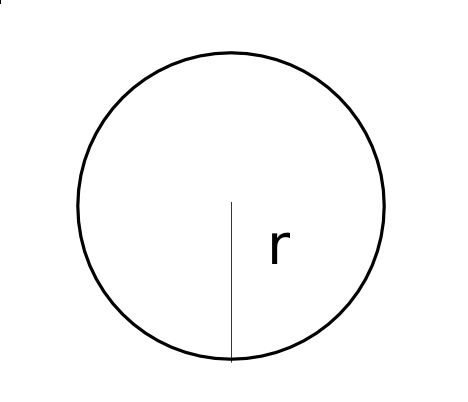
\includegraphics[width=0.5\textwidth]{./images/wheel_r}
\caption{koło robota}
\label{wheel_r}
\end{figure}


gdzie:

\begin{itemize}
    \item $k$ -- rozdzielczość enkodera (ilość impulsów na obrót)
    \item $r$ -- promień koła
    \item $x$ -- ilość impulsów odczytywanych z enkodera podczas przejazdu
\end{itemize}

Podczas jazdy do przodu niezbędne jest dbanie o to aby robot poruszał się po zadanej trajektorii. Jak wcześniej wspomniano problemem jest również kontrola orientacji robota podczas jazdy do przodu. Poprzez sterowanie wypełnieniem sygnału przekazywanym na silniki nie można zapomnieć o tym że różnią się one między sobą. Skutkuje to tym że po zadaniu takiego samego wypełniania sygnału sterującego prędkością obrotową silników, mogą one przebyć różne drogi. 

Ponadto masa robota również nie jest rozłożona równomiernie w wyniku czego nacisk wywierany na koła robota jest różny. Przekłada się to na różną siłę tarcia jaką muszą pokonać koła robot. W tym przypadku również przy zadaniu takiego samego sygnału sterującego silnikami mogą one przebyć różne drogi.

Przytoczone problemy można wyeliminować poprzez kontrolę drogi przejechanej przez obydwa koła i odpowiednią korekcję sygnału sterującego. 


\chapter{Narzędzia} 

\section{Czujniki} 
W robocie wykorzystano następujące czujniki, które umożliwił prawidłową nawigację robota w labiryncie:

\subsubsection{Żyroskop L3GD20} % (fold)
    Został on wykorzystany do pomiaru pomiaru orientacji robota. L3GD20 jest żyroskopem 3 osiowym jednakże pomiary dokonywane są tylko w jednej osi ze względu na to, że robot nie ma możliwości poruszania się wokół dwóch pozostałych. Żyroskop można skonfigurować tak aby wybrać zakres pomiarów dopasowany do potrzeb użytkownika. Po licznych testach zdecydowano się na zakres 2000 dps ze względu na znaczne prędkości kątowe jakie osiągał robot. Zastosowany w żyroskopie interfejs SPI jest bardzo szybki i praktycznie nie wprowadza on opóźnień do pętli sterowani. Zastosowany żyroskop charakteryzuje się małym dryfem co pozwala robotowi na dłuższą niż w przypadku gorszych jakościowo żyroskopu pracę bez kalibracji, jednak tak jak w każdym żyroskopie jego wpływ jest w końcu odczuwalny. Przy wyborze żyroskopu kierowano się tym, aby pomiar był realizowany poprzez sygnał cyfrowy minimalizuje to występowanie zakłóceń związanych z pomiarem sygnału analogowego i zakłócaniu go poprzez inne elementy znajdujące się na płytce robota, wiązało się to również z brakiem konieczności posiadania stabilnego napięcia referencyjnego na płytce. 

\begin{figure}[h]
\centering
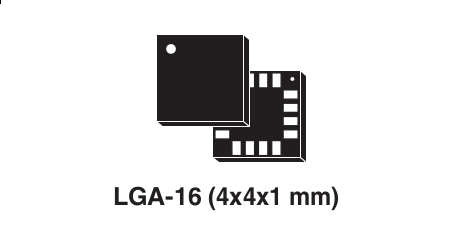
\includegraphics[width=0.7\textwidth]{./images/L3GD20}
\caption{Żyroskop L3GD20}
\label{L3GD20}
\end{figure}


\subsection{Enkoder magnetyczny MEMS4020}

Wspomniany enkoder wykorzystano do pomiaru drogi przejechanej przez robota oraz do kontroli trajektorii po jakiej poruszał się robot.  Wspomniany enkoder dysponuje 3 różnymi zakresami dla robota klasy Micromouse wystarczył najmniejszy z możliwych zakresów tj. 512 ticków na obrót co pozwoliło robotowi na wystarczająco dokładny pomiar. Wybrany żyroskop jest niewielki i świetnie sobie radzi nawet gdy magnes nie jest zamontowany idealnie nad nim. Do komunikacji z żyroskopem spośród trzech opcji :
\begin{itemize}
    \item SPI
    \item I2C
    \item Wyjście kwadraturowe
\end{itemize}

Wybrano ostatnią opcję ze względu na sprzętową obsługę tego typu sygnału przez mikrokontroler.

\begin{figure}[h]
\centering
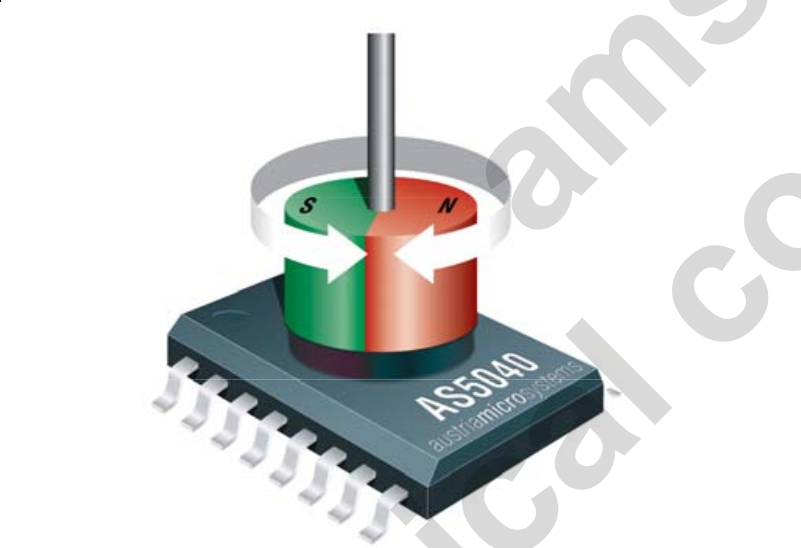
\includegraphics[width=0.8\textwidth]{./images/MEMS4020}
\caption{MEMS4020}
\end{figure}

\subsection{Czujnik optyczny na bazie fotodiody i fototranzystora}

    Ze względu na brak gotowych dostępnych czujników odległości, które posiadałyby wymagany zakres pomiarów (2-35cm) zdecydowano się na zaprojektowanie własnych czujników opartych o fotodiodę i fototranzystor. Światło które pochodzi z fotodiody odbija się od ścian labiryntu, a następnie pada na fototranzystor. Napięcie które pojawia się na wyjściu fototranzystora jest odwrotnie proporcjonalne do odległości czujnika od ściany. Fotodioda jest załączana okresowo co umożliwia pobudzanie jej większym prądem niż w przypadku pracy ciągłej. Większy prąd skutkuje tym, że dioda świeci mocniej co pozwala na wykonywania pomiaru z większej odległości Dodatkowo możliwe jest wykonanie pomiaru różnicowego. Ponieważ możemy zmierzyć poziom światła widzialnego jakie pobudza fototranzystor przy zgaszonej diodzie i użyć tych danych do filtracji pomiaru. Zdecydowano się na wybór:

\begin{itemize}
        \item diody IR LD271 
        \item fototranzystora SFH313
\end{itemize}
    
\begin{figure}[h]
\centering
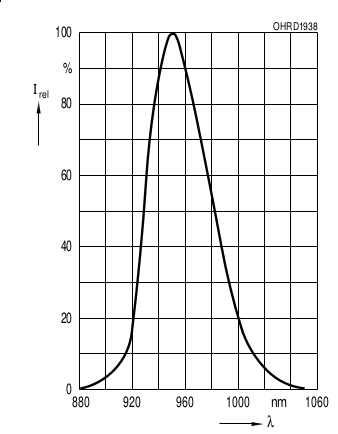
\includegraphics[width=0.3\textwidth]{./images/diodair}
\caption{Charakterystyka diody Ir}
\label{diodair}
\end{figure}

\begin{figure}[h]
\centering
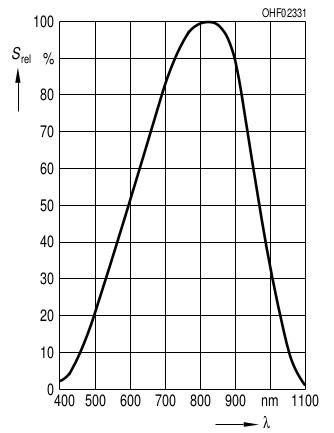
\includegraphics[width=0.3\textwidth]{./images/fototranzystor}
\caption{Charakterystyka fototranzystora}
\label{fototranzystor}
\end{figure}

Ze względu na przedział długości fal jakie generuje dioda IR, które wpasowują się w charakterystykę fototranzystora.
    
Wybrany zestaw pozwala na pomiar odległości robota od ścian w zakresie 2-35 cm. Jest to wynik wystarczający, który pozwala robotowi na odpowiednio szybkie wykrycie obecności ściany labiryntu i umożliwia mu wyhamowanie przed nią. 

\section{Filtracja i fuzja pomiarów} % (fold)
Robot dysponuje różnego rodzaju czujnikami. Każdy pomiar obarczony jest zakłóceniami wynikającymi z dalekiego od ideału działania przyrządów pomiarowych dlatego też wymagane jest przygotowanie odpowiednich algorytmów pozwalających na filtrację takich pomiarów.

Występuje również konieczność przeprowadzenia fuzji pomiarów ponieważ sensory pozwalając na pomiar jednego parametru robota na kilka różnych sposobów w tym celu rozważono możliwe rozwiązania i zdecydowano się na wybór optymalnych.


\subsection{Filtracja pomiarów pochodzących z czujnika odległości} 
\subsection{Filtracja pomiarów pochodzących z żyroskopu} 
\subsection{Filtracja pomiarów pochodzących z enkoderów} 

\subsection{Fuzja sygnałów podczas obrotu robota w miejscu} 
Żyroskop jest inercyjnym sensorem, który idealnie nadaje się do pomiaru orientacji, poprzez całkowanie prędkości kątowej wokół osi Z, której wartość odczytywana jest z żyroskopu. Jednocześnie całkowany jest błąd tzw dryf. Skutkuje to tym, że po pewnym czasie pozycja mierzona może znacznie różnić się od pozycji rzeczywistej robota. W celu kalibracji czujnika i kompensacji błędów możliwe jest wykorzystanie np. filtru Kalmana jednakże wprowadza on przesunięcie fazowe do pomiarów co również jest zjawiskiem nie pożądanym.


Istnieją konstrukcje robotów klasy Micromouse, które nie wykorzystują żyroskopów, a wszelkie informacje o orientacji oszacowują za pomocą pomiarów z enkoderów. Jednakże pomiar orientacji robota przy wykorzystaniu żyroskopu jest o wiele bardziej dokładny. W celu minimalizacji wpływu dryfu żyroskopu na pomiary można włączać żyroskop jedynie na czas obrotu w miejscu i wyłączać go gdy robot osiągnie zadaną orientację. Warunkiem działania tego typu algorytmu jest dobrze określona orientacja robota przed pokonaniem zakrętu. Za pomocą żyroskopu możliwy jest pomiar względnej zmiany orientacji względem pozycji startowej. Powinno to znacząco poprawić jakość sterowania względem wykorzystania samych enkoderów. 

\subsection{Fuzja sygnałów przy utrzymywaniu orientacji robota podczas jazdy wzdłuż prostej} 

Dla robotów klasy Micromouse niezwykle ważne jest utrzymywanie zadanej orientacji robota podczas jazdy do przodu, przy wykorzystanej w robocie sensoryce może być to realizowane na co najmniej kilka sposobów. Do pomiaru przejechanej drogi wykorzystywane są enkodery magnetyczne. 

W celu wymuszania na robocie jazdy po linii prostej możliwa jest kontrola i minimalizacja w czasie rzeczywistym różnicy dróg jaką pokonują koła robota. Taki algorytm sterowania może przynosić dobre rezultaty jednakże jest on wrażliwy na zjawisko poślizgów kół robota. 

Alternatywnym rozwiązaniem jest kontrola orientacji robota za pomocą żyroskopu jednakże, jak wcześniej wspomniano wiąże się z tym potrzeba kompensacji dryfu. W przypadku wykorzystania pomiarów z żyroskopu przy sterowaniu obrotem robota w miejscu założyliśmy, że proces regulacji będzie na tyle krotki, że dryf można pominąć oraz że pozycja początkowa dobrze określona. Sformułowanie takiego samego założenia dla kontroli orientacji robota podczas jazdy do przodu byłoby niepoprawne ze względu na drugie z założeń. Wedle niego pozycja początkowa ruchu obrotowego w miejscu musi być dobrze określona, jeżeli jej wartość będzie zależeć bezpośrednio od pomiarów z żyroskopu, które obarczone są błędem wynikającym z dryfu żyroskopu nie zagwarantuje to  spełnienia tego założenia. Pozostawienie algorytmu sterowania w takiej postaci skutkuje nawarstwianiem się z czasem błędów wynikających z dryfu żyroskopu, który nie jest w żadnym miejscu kompensowany. 

Brakującym fragmentem algorytmu regulacji jest brak kompensacji dryfu żyroskopu. Spotkać się można z kilkoma powszechnie polecanymi rozwiązaniami:

\begin{itemize}
    \item wykorzystując filtr Madgwicka,
    \item wykorzystując filtr Kalmana,
    \item wykorzystując odczyty z czujników odległości.
\end{itemize}

\subsubsection{Filtr Madgwicka} 
    Filtr Madgwicka jest stosunkowo nowym filtrem, który przy wykorzystaniu żyroskopu, akcelerometru i magnetometru pozwala na określenie orientacji robota w przestrzeni. Bazuje on głównie na żyroskopie, a dodatkowe czujniki wykorzystywane są do kompensacji dryfu żyroskopu. Zastosowanie go idealnie nadawało by się do odfiltrowanie zakłóceń spowodowanych przez dryfu żyroskopu, jednakże do działania wymaga on zastosowanie magnetometru, który nie został wykorzystany w przygotowanym prototypie robota. 

\subsubsection{Filtr Kalmana} 
Można spotkać się z opiniami, że do kompensacji dryfu żyroskopu nadaje się wykorzystanie filtru Kalmana co nie do końca jest prawdą. Filtr ten może być wykorzystywany do wygładzania charakterystyk pochodzących z pomiarów lecz sam w sobie nie potrafi poradzić sobie z dryfem żyroskopu, wymagane jest zastosowanie dodatkowego czujnika. Filtr Kalmana można wykorzystać dla układu pomiarowego, który już taką fuzję realizuje. Poskutkowałoby to uzyskaniem stabilnych pomiarów np. w stanie spoczynku gdy robot się nie porusza przy dobrze nastrojonym filtrze odczyty również byłyby stałe. Dryf żyroskopu ma stałą wartość, która nawarstwia się wraz z całkowaniem pomiarów. 

Poprzez filtrowanie pomiarów z samego żyroskopu uzyskalibyśmy jedynie bardziej gładką charakterystykę z ograniczoną ilością szumów pomiarowych. Wykorzystany L3GD20 posiada 10 bitowy w celu eliminacji szumów wystarczy pominąć kilka pierwszych bitów przy pomiarze. Dla robota omawianej klasy dokładność takiego pomiaru i tak będzie zadowalająca.

\subsubsection{Kompensacja dryfu za pomocą czujników odległości} 
Aby skompensować dryf po rozważeniu innych opcji zdecydowano się na wykorzystanie do tego celu czujników odległości. Wykonane czujniki na wyjściu mają sygnał analogowy odwrotnie proporcjonalny do odległości od ścian labiryntu. 
W celu usunięcia dryfu wykorzystywany jest pomiar odległości robota od ścian labiryntu. Ze względu na to że podczas startu robot umieszczany jest w polu z którego istnieje tylko jedna droga wyjazdu możliwe jest wykonanie pomiaru wartości zwracanych przez czujniki odległości od ścianek znajdujących się po bokach robota. Wykonywana jest seria pomiarów próbnych z czujników, a następnie odrzucone zostają skrajne pomiary z próby-- z pozostałych zostaje wyznaczona wartość średnia. Pomiary uzyskane w ten sposób są pomiarami referencyjnymi. Ze względu na to że rozmiary pola labiryntu są takie same robot może starać się kalibrować swoją orientację przy każdej okazji gdy po jego bokach znajdują się ściany labiryntu. W wyniku takiego działania algorytmu dryf żyroskopu może być kompensowany na tyle często aby możliwa była zaawansowana eksploracja labiryntu a w skrajnym przypadku jego przegląd zupełny.
\chapter{Metoda lokalizacji} % (fold)

\section{Dwu warstwowy interfejs algorytmu} 
\subsection{Lokalizacja z dokładnością do komórki labiryntu} 
\subsection{Lokalizacja robota względem środka danej komórki} 

\chapter{Konstrukcja robota} % (fold)
\section{Software} 
\section{Hardware} 
\section{Mechanika} 
\chapter{Badania} % (fold)
\section{Porównanie jakości sterowania orientacją robota przy wykonywaniu obrotu w miejscu} 
\subsection{Żyroskop} 
\subsection{Enkoder} 
\section{Porównanie jakości sterowania orientacją robota przy poruszaniu się po lini prostej} 
\subsection{Żyroskop} 
\subsection{Enkoder} 
\subsection{Fuzja sygnałów} 
% section  (end)
% section  (end)
\chapter{Wnioski} % (fold)
\label{cha:Wnioski}

% chapter Wnioski (end)
\label{cha:Badania}

% chapter Badania (end)
% section  (end)
% section  (end)
% section  (end)
% section  (end)
\label{cha:Konstrukcja robota -}

% chapter Konstrukcja robota - (end)

% section  (end)
% section Filtracja pomiarów (end)

%\bibliographystyle{plabbrv}
%\bibliography{bibliografia}

\end{document}
